\section{Installation and setup}
\subsection{General requirements}
\subsubsection{Hardware requirements}
The only hardware required is to own a CPU newer than a Pentium 4 with SSE2 instruction set. 
\subsubsection{Software requirments }
This application can run on GNU/Linux on any distribution newer than Ubuntu 14.04, MacOs from 10.10 onward and Windows from 7 and onward; Other than an operative system this application needs: 
\begin{itemize}
	\item \textbf{Node.js}: version 10.16.3 (or higher) to be installed on your system. To install it, the user can refer to the official web page nodejs.org for installation we recommend the LTS version;
	\item \textbf{npm}: Node Package Manager (npm) version 6.9.0 (or higher) is the package manager that comes with Node.Js; 
	\item \textbf{TypeScript}: to install TypeScript\glo the user needs to run npm install typescript -g, the 
minimum version required is the 3.6.5; 
	\item \textbf{ts-node}: to install ts-node the user needs need to run npm install ts-node -g, this operation will install globally the command ts-node; 
%	\item Having an \textit{Ethereum\glo} account on the network Ropsten with an amount of credit inside.
\end{itemize}
For simplicity the user can install multiple packages in one command.\\\\
\centerline{\code{Install typescript ts-node -g}}\\\\
After entering the command, the CLI should look like the picture.

\begin{figure}[h]
	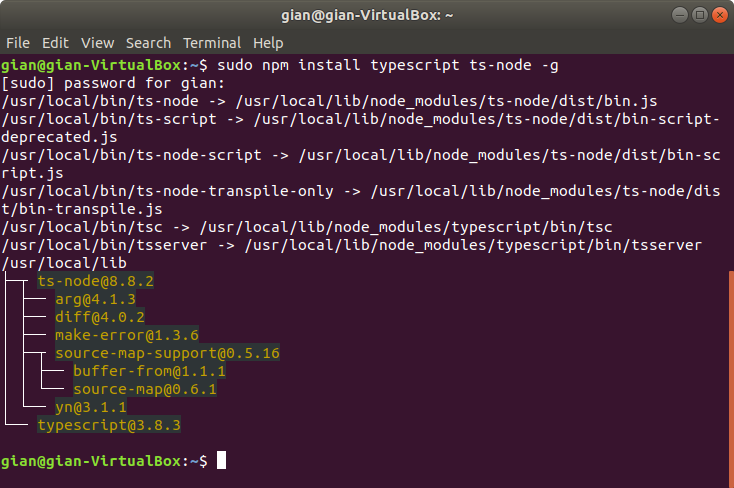
\includegraphics[width=\textwidth]{res/img/typescriptInstall.png}
	\caption{Typescript Install}
\end{figure}
\newpage
\subsection{Etherless-cli}
\subsubsection{Setup}
To install Etherless-cli is sufficient to start the installation process\\\\
\centerline{\code{run npm install –dotenv-extended}}\\\\
To check if the setup completed correctly, the user can run the unit test.\\\\
\centerline{\code{npm run test}}\\\\
If the output of the command looks like the example than the installation was successful.\\
\begin{figure}[h!]
	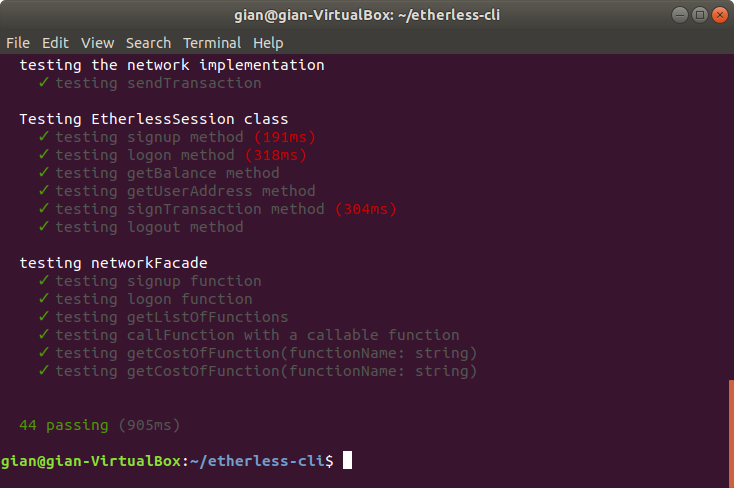
\includegraphics[width=\textwidth]{res/img/npmruntest.png}
	\caption{Run test}
\end{figure}\\
\newpage
\noindent Before starting to use the software the user needs to register an Ethereum account or login with an already existing one, after the that the user needs to add funds to the wallet. The user can do that by importing the new account in MetaMask\glo.
\subsubsection{Run}
To run this program from the command line interface positioning on the main program folder and type ts-node . «command» where «command» is the command that the user wants to run.
%To download and install the application it is necessary to open the terminal/shell of your operating system and write the command \\
%\centerline{\code{npm install etherless-cli -g}}\\
%\begin{figure}
%	\centering
%	\includegraphics[width=\textwidth]{res/img/Screenshot_etherless_install.jpg}
%	\caption{command list}
%\end{figure}
%aggiungere uno screen
%Once installed the user must be able to perform the following commands by CLI\glo: 
%\begin{itemize}
%	\item init;
%	\item signup;
%	\item login;
%	\item logout;
%	\item list;
%	\item find;
%	\item create;
%	\item run;
%	\item log;
%	\item update;
%	\item delete.
%\end{itemize}